\documentclass[10pt, a4paper, onecolumn, final]{article}
% 3 pacotes para hifenização correta em português.
\usepackage[brazilian]{babel}
\usepackage[utf8]{inputenc}
\usepackage[T1]{fontenc}
%Para excluir o recuo do 1o paragrafo
\usepackage{parskip}
%Para inserir figuras
\usepackage{graphicx}
\usepackage{amsmath}
%\usepackage[all]{xy}
%\usepackage[]{geometry} %top=1cm, bottom=0cm,left=3.5cm, right=3.0cm
\usepackage{amssymb}
\usepackage{textcomp} %para o sinal de copyright 
\title{Matrizes, Sistemas Lineares\\ e \\Determinantes}
\author{Roberto Kahn Pereira}
\date{Julho/2012}

%\includeonly{introducao}
%\includeonly{operacoesComMatrizes}
%\includeonly{inversa}
%\includeonly{sistemas}
%\includeonly{determinantes}

\begin{document}
\maketitle
\vfill
\newpage
\tableofcontents
\newpage
\section*{Agradecimentos}
\addcontentsline{toc}{section}{Agradecimentos}
Agradeço a Deus por me dar inteligencia e meios para escrever trabalhos como este. Este trabalho foi escrito em \LaTeX, usando o software LaTeXila em um PC com sistema Ubuntu. Um agradecimento a todos os envolvidos nesses projetos.
\section*{Licença}
\addcontentsline{toc}{section}{Licença}
Este trabalho foi licenciado com a Licença Creative Commons Atribuição - Não Comercial 3.0 Brasil. Para ver uma cópia desta licença, visite:\\http://creativecommons.org/licenses/by-nc/3.0/br/\\ ou envie um pedido por carta para Creative Commons, 444 Castro Street, Suite 900, Mountain View, California, 94041, USA.\\
Você tem a liberdade de:
\begin{description}
    \item[Compartilhar] copiar, distribuir e transmitir a obra.
    \item [Remixar] criar obras derivadas.
\end{description}
Sob as seguintes condições:
\begin{description}
    \item[Atribuição] Você deve creditar a obra da forma especificada pelo autor ou licenciante (mas não de maneira que sugira que estes concedem qualquer aval a você ou ao seu uso da obra).
    \item[Uso não comercial] Você não pode usar esta obra para fins comerciais.
\end{description}
Comentários e sugestões, posso ser encontrado em: robertokahn@facebook.com\\
Código e arquivos dvi e ps disponiveis em:\\http://github.com/BetoKahn/Matrizes\\[0.5cm]
%\begin{center}
    \textcopyright 2012 Roberto Kahn Pereira
%\end{center}
\section*{Sobre este texto}
\addcontentsline{toc}{section}{Sobre este texto}
Quando eu dava plantão de dúvidas em um cursinho, percebi que precisava estudar mais sobre determinantes. A motivação para esse estudo foi começar a escrever um texto sobre o assunto, e como eu queria aprender \LaTeX, comecei a escrever nessa linguagem. Usei a sequência de temas: matrizes, sistemas e determinantes, porque me pareceu mais simples dessa forma.\\
O conteúdo aborda quase todos os temas dados no ensino médio, mas acredito que possa ser usado como um resumo desses temas para cursos introdutórios de álgebra linear e vetores ou calculo numérico. Alguns temas estão faltando como: Sistemas de Cramer e determinação da inversa através da matriz adjunta e talvez algum outro tema que não me lembre agora.\\
Espero que você goste do trabalho, no futuro pode ser que eu complete os temas faltantes.
\newpage
\hangindent=0.0cm
\section{Introdução}
As matrizes são agrupamentos de números reais ou complexos organizados de forma ordenada em linhas e colunas e delimitados por grandes colchetes [] ou parenteses() . São objetos matemáticos com grande importância em física e matemática, como por exemplo, na matemática vetorial ou em problemas de mecânica dos corpos rígidos e em mecânica quântica e relatividade. As matrizes possuem propriedades importantes de se conhecer sobre as quais falarei neste trabalho.\\
Algumas definições de notação:
\begin{itemize}
  \item As matrizes são denotadas por letras maiúsculas. Ex. A letra \textbf{A} representa a matriz A.
  \item O número de linhas e colunas de uma matriz é escrito em subscrito junto ao nome da matriz. Exemplo: $A_{2\times3}$ significa que a matriz A possui 2 linhas e 3 colunas.
  \item Um elemento de uma matriz é denotado pela letra da matriz em forma minuscula com o número da linha e coluna (nessa ordem, sempre) em sobrescrito. Por exemplo, $a_{11}$ é o elemento da linha 1 e coluna 1 da matriz A.
  \item De forma mais genérica denotamos $a_{ij}$ o elemento da linha i e coluna j da matriz A.
\end{itemize}  

\paragraph*{Matriz retangular} é o tipo mais genérico de matriz, que possui número de linhas diferente do número de colunas. Um exemplo de matriz retangular:
\begin{displaymath}
\begin{bmatrix}
  1 & 2 & 3 \\  4 & 5 & 6
\end{bmatrix}.
\end{displaymath}

\paragraph*{Matriz quadrada} é uma matriz que possui o mesmo número de linhas e colunas, esse número é chamado de \textit{ordem} da matriz. A matriz $B_{2\times2}$ é dita de ordem 2 e pode ser escrita como $B_{2}$.Um exemplo de matriz quadrada de ordem 2:
\begin{displaymath}
\begin{bmatrix}
  2 & 4 \\ \pi & sen(30^0)
\end{bmatrix}
\end{displaymath}
\paragraph*{A Diagonal principal} de uma matriz quadrada A de ordem m $A_m$ são os elementos $a_{ij}$ tais que i=j ($a_{11},\, a_{22},\, a_{33},...$. Na matriz $4 \times 4$ a seguir a diagonal principal contem o símbolo **:
\begin{displaymath}
\begin{pmatrix}
** & 2 & 3 & 7\\
1 & ** & 34 & 3\\
34 & 6 & ** & 12\\
8,7 & 1 & 1 & ** \\
\end{pmatrix}
\end{displaymath}
\paragraph*{A Diagonal secundaria} da matriz $A_m$ é a diagonal que começa em $ a_{1m} $ e termina em $ a_{m1} $, indicada na matriz $ 3 \times 3 $ a seguir por **:
\begin{displaymath}
\begin{pmatrix}
1 & 2 & **\\
0 & ** & 5 \\
** & 4 & 7
\end{pmatrix}
\end{displaymath}
\paragraph{A Matriz transposta} de uma matriz $A_{m\times n}$ é a matriz $(A^t)_{n\times m}$, tal que
o elemento $(a^t)_{ij}$ da transposta é o elemento $(a_{ji})$ da matriz original, ou seja, as linhas de A viram as colunas da transposta.
Para uma matriz $A_{2 \times 3}$ genérica:
\begin{displaymath}
  A=
  \begin{bmatrix}
  a_{11} & a_{12} & a_{13} \\ 
  a_{21} & a_{22} & a_{23}
  \end{bmatrix}
  \; A^t=
  \begin{bmatrix}
  a_{11} & a_{21} \\ 
  a_{12} & a_{22} \\
  a_{13} & a_{23}
  \end{bmatrix}
\end{displaymath}
Um exemplo prático, a transposta da matriz $A_{2 \times 2}$ dada a seguir:
\[ A=
\begin{bmatrix}
1 & 2 \\ 3 & 4 \\
\end{bmatrix}
 \; A^t=
 \begin{bmatrix}
   1 & 3 \\ 2 & 4 \\
 \end{bmatrix}
 \]

\section{Operações com matrizes}
\subsection{Multiplicação por Real}
Para multiplicar uma matriz A por um numero real $\alpha$, se deve multiplicar todos os elementos da matriz por $\alpha$, como a seguir:
\begin{displaymath}
\text{Seja a matriz A=}
\begin{bmatrix}
  a_{11} & a_{12}\\ a_{21} & a_{22}\\ a_{31} & a_{32}\\
\end{bmatrix}
\end{displaymath}
e seja $\alpha$ um número real qualquer, então:
\begin{displaymath}
\alpha \cdot A = \begin{bmatrix}
  \alpha \cdot a_{11} &\alpha \cdot  a_{12}\\ \alpha \cdot a_{21} &\alpha \cdot  a_{22}\\
  \alpha \cdot a_{31} & \alpha \cdot a_{32} \end{bmatrix}
\end{displaymath}
Em relação a multiplicação de uma matriz por um número real, vale a propriedade comutativa: \[A \cdot \alpha = \alpha \cdot A \]
Exemplo: Seja $ A= \left( \begin{smallmatrix} 11 & 26 \\ \pi & 5
\end{smallmatrix} \right)$. Calcular a matriz B, tal que $B=3A$.
%\begin{align*}
\begin{displaymath}
B=3A=3 \cdot
  \begin{bmatrix}
    11 & 26 \\ \pi & 5
  \end{bmatrix}
  =
  \begin{bmatrix}
    3 \cdot 11 & 3 \cdot 26 \\ 3 \cdot \pi & 3 \cdot 5
  \end{bmatrix}
  =
  \begin{bmatrix}
    33 & 78 \\ 3\pi & 15
  \end{bmatrix}
\end{displaymath}
%\end{align*}
\subsection{Soma e subtração}
A soma (e subtração) de matrizes se faz assim: Basta somar ( ou subtrair ) um a um os elementos das duas matrizes.
Sejam A e B duas matrizes e C = A + B, resulta $c_{ij}=a_{ij}+b_{ij}$.\\
Para simplicidade vou usar matrizes $2 \times 2$, mas muitas dessas operações valem para matrizes $n \times m$. Para matrizes genéricas $2 \times 2$ fica:
\begin{displaymath}
  A+B=
  \begin{bmatrix}
  a_{11} & a_{12}\\a_{21} & a_{22}  
  \end{bmatrix}
  +
  \begin{bmatrix}
  b_{11} & b_{12}\\b_{21} & b_{22}  
  \end{bmatrix}
  =
  \begin{bmatrix}
  a_{11}+b_{11} & a_{12}+b_{12}\\a_{21}+b_{21} & a_{22}+b_{22}  
  \end{bmatrix}
\end{displaymath}
Exemplo:
\begin{displaymath}
A=
\begin{bmatrix}
  1 & 2 \\ 3 & 4
\end{bmatrix}
 \quad B=\begin{bmatrix}
 5 & 6 \\ 7 & 8 \end{bmatrix}
\quad A + B =
\begin{bmatrix}
  1+5=6 & 2+6=8\\
  3+7=10 & 4+8=12
  \end{bmatrix}
\end{displaymath}
Fazendo agora a subtração $ B-A $, temos:
\begin{displaymath}
\begin{bmatrix}
5 & 6 \\
7 & 8
\end{bmatrix}
-
\begin{bmatrix}
1 & 2 \\ 
3 & 4
\end{bmatrix}
=
\begin{bmatrix}
5-1 & 6-2 \\ 
7-3 & 8-4
\end{bmatrix}
=
\begin{bmatrix}
4 & 4 \\ 
4 & 4
\end{bmatrix} 
\end{displaymath}
Para a adição de matrizes valem as propriedades:
\begin{description}
\item[Comutativa] $A+B=B+A$
\item[Associativa]$ A+(B+C)=(A+B)+C $
\end{description}

\subsection{Multiplicação}
A multiplicação de matrizes é um pouco mais complicada. Primeiro: O número de colunas da primeira matriz deve ser igual ao número de linhas da segunda, sem essa condição não é possivel a multiplicação de matrizes e com alguma prática, você entenderá porque. 
Suponha duas matrizes quadradas 2x2 A e B, a multiplicação A$\cdot$B=P, resulta: 
\begin{displaymath}
\begin{bmatrix}
  a_{11} & a_{12}\\ a_{21} & a_{22}\\
\end{bmatrix}
\cdot
\begin{bmatrix}
  b_{11} & b_{12}\\ b_{21} & b_{22}\\
  \end{bmatrix}
=
\begin{bmatrix}
  a_{11}b_{11}+a_{12}b_{21} & a_{11}b_{12}+a_{12}b_{22} \\
  a_{21}b_{11}+a_{22}b_{21} & a_{21}b_{12}+a_{22}b_{22} \\
\end{bmatrix}
 =
\begin{bmatrix}
   p_{11} & p_{12} \\ p_{21} & p_{22} \\
\end{bmatrix}
\end{displaymath}
Agora você viu que o termo $p_{ij}$ se calcula a partir da linha i da matriz A e da coluna j da matriz B, se deve multiplicar termo a termo e somar os produtos dos elementos dessas linhas e colunas. Observe que a multiplicação de matrizes não é necessariamente comutativa, ou seja, $A\cdot B$ pode ser diferente de $B\cdot A$. Não existe divisão de matrizes.\\
Exemplo:\\
Sejam as matrizes:
\begin{displaymath}
  A=
  \begin{bmatrix}
    1 & 3 \\ 5 & 7
  \end{bmatrix}
  \text{ e }
  B=
  \begin{bmatrix}
    2 & 4 \\ 6 & 8
  \end{bmatrix}
\end{displaymath}
O produto $A \cdot B$ é:
\begin{displaymath}
A\cdot B=
\begin{bmatrix}
  1 \cdot 2+3 \cdot 6 & 1 \cdot 4+3 \cdot 8 \\
  5 \cdot 2+7 \cdot 6 & 5 \cdot 4+7 \cdot 8
\end{bmatrix}
=
\begin{bmatrix}
  20 & 28\\
  52 & 76
\end{bmatrix}
\end{displaymath}
O produto $B\cdot A$ resulta:
\begin{displaymath}
  B\cdot A=
  \begin{bmatrix}
    22 & 34\\46 & 74
  \end{bmatrix}
\end{displaymath}
Você pode fazer a demonstração como exercício.

\section{Matriz Inversa}
\subsection{Matriz Identidade}
Existe uma matriz especial, chamada \textit{matriz identidade}. Normalmente ela é denotada pela letra I, e ela é sempre quadrada com o número 1 na diagonal principal e 0 no resto. Ex:
\begin{displaymath}
I_2=
\begin{bmatrix}
1 & 0 \\
0 & 1 \\
\end{bmatrix}
\: I_3=
\begin{bmatrix}
1 & 0 & 0 \\ 0 & 1 & 0 \\ 0 & 0 & 1\\
\end{bmatrix}
\end{displaymath}
\subsection{Matrizes Equivalentes}
 Sejam M, M' e M'' matrizes equivalentes, elas possuem as seguintes propriedades:\\
O Sinal $\sim$ indica uma relação de equivalência\footnote{Esse tópico é objeto de estudo da álgebra e tem importância também no estudo de sistemas lineares. Sistemas lineares são vistos na seção \ref{sec:sis}.}. Achei interessante mencionar esse assunto para mostrar que há relação entre uma matriz (ou sistema) que sofre uma operação elementar e a matriz, ou sistema, resultante dessa operação, porque apesar de não serem identicos, possuem entre si uma relação de equivalencia, que garante certas propriedades.
\begin{description}
  \item[Reflexiva] M $\sim$ M.
  \item[Simétrica] $M\sim M'\Rightarrow M'\sim M.$
  \item[Transitiva]$Se\,  M\sim M'\text{ e }M'\sim M''\text{, então }M\sim M''.$
\end{description}
\subsection{Operações elementares}
\label{subsec:ope-ele}
Existem 3 operações que se pode fazer com as linhas de uma matriz M e transformam M em M' que é equivalente à M, essas operações são chamadas de \textit{operações elementares}. 
As operações elementares são:
\begin{enumerate}
  \item Trocar duas linhas de uma matriz entre si. Por exemplo:$
  \begin{bmatrix}
  1 & 2 \\ 3 & 4  
  \end{bmatrix}
  \sim
  \begin{bmatrix}
    3 & 4 \\1 & 2
  \end{bmatrix}
  $
  \item Multiplicar uma linha por um número diferente de 0.
  \item Multiplicar uma linha por um número diferente de 0 e somar a outra linha.
\end{enumerate}
\subsection{Definição de Matriz Inversa}
A matriz inversa de A é a matriz $A^{-1}$, tal que $A\cdot A^{-1}=A^{-1}\cdot A = I$. Se existe A e $A^{-1}$, então é dito que a matriz A é \textit{inversível}, mas cuidado, porque nem toda matriz é inversível. Mais a frente será visto um algoritmo (método) para se obter a inversa de uma matriz.\\
Uma matriz com determinante\footnote{Os determinantes são vistos mais a frente na seção \ref{sec:det}.} nulo \textit{não é inversível}. Se uma matriz possui uma linha (ou coluna) inteira nula (somente com o número 0), ou se ela possui 2 linhas ou colunas iguais, então ela possui determinante nulo e \textit{não possui inversa}.
\subsection{Determinação da Inversa}
Existe um teorema que garante que o mesmo conjunto de operações elementares que transformam $A$ em $I$, também transformam $I$ em $A^{-1}$, caso exista. Então basta escrever a Matriz $A$ ao lado da $I$, separadas por um traço vertical para melhor vizualização, e aplicar operações elementares\footnote{Aquelas operações definidas em \ref{subsec:ope-ele}} simultaneamente na atriz $A$ e na $Identidade$ até que $A$ se torne a $Identidade$, então do outro lado estará a inversa. Exemplo:
\begin{displaymath}
\text{Seja A=}
\begin{bmatrix}
  1 & 0 \\ 3 & 4
\end{bmatrix}
\end{displaymath}
Vamos calcular a matriz $A^{-1}$:
\begin{displaymath}
\left(
\begin{array}{c c|c c}
  1 & 0 & 1 & 0\\3 & 4 & 0 & 1
\end{array}\right)
\end{displaymath}
Dividindo por 4 a $2^a$ linha, resulta:
\begin{displaymath}
\left(\begin{array}{c c|c c}
  1 & 0 & 1 & 0\\3/4 & 1 & 0 & 1/4
\end{array}\right)
\end{displaymath}
Multiplicando a $1^a$ linha por -3/4 e somando com a $2^a$, obtemos o resultado final:
\begin{displaymath}
\left(\begin{array}{c c|c c}
  1 & 0 & 1 & 0\\0 & 1 & -3/4 & 1/4
\end{array}\right)
\end{displaymath}
Do lado esquerdo temos a matriz identidade e do direito a inversa da matriz inicial.
A matriz $A^{-1}$ resulta:
\begin{displaymath}
A^{-1}=\begin{bmatrix}
  1 & 0 \\ -3/4 & 1/4
\end{bmatrix}
\end{displaymath}
%Escrever método dos cofatores

\section{Sistemas Lineares}
\label{sec:sis}
Um sistema linear é qualquer agrupamento de equações com variáveis de expoente 1, como por exemplo:
\begin{displaymath}
\left\{
\begin{array}{l}
  3x+y=1\\2x+5y=3
\end{array}
\right.
\end{displaymath}
Um sistema pode ter, a principio, qualquer número de variáveis e equações, como veremos mais a frente.
Um sistema linear pode ser expresso de forma matricial. Usando o sistema do exemplo anterior, podemos re-escreve-lo como:
\[
\begin{bmatrix}
  3 & 1\\2 & 5 \end{bmatrix}
\cdot
\begin{bmatrix}
  x\\y \end{bmatrix}
=
\begin{bmatrix}
  1\\3 \end{bmatrix}
  \]
  Todo sistema linear pode ser escrito como $A\cdot X=B$, onde A é chamada de \textit{matriz dos coeficientes}, X é chamada de \textit{matriz das incógnitas} e B é chamada de \textit{matriz dos termos independentes}.
  
  Em sistemas se podem aplicar operações elementares às equações do sistema, de forma idêntica ao que se pode fazer com matrizes e o sistema resultante será um sistema equivalente, com as mesmas propriedades da equivalência de matrizes.
  \[\text{O sistema:}\left\{
  \begin{array}{l}
    3x+2y=4\\ 5x+y=3
  \end{array}\right.
  \sim
  \left\{
  \begin{array}{l}
    3x+2y=4\\ 2x-y=-1
  \end{array}\right.\]
  Onde subtrai a $2^a$ equação da $1^a$ e o sinal $\sim$ representa a relação de equivalência.
  \subsection{Resolução de Sistemas Lineares}
\subsubsection*{Método da substituição}
  \addcontentsline{toc}{subsubsection}{Método da substituição}
  Resolver um sistema linear significa determinar o valor das incógnitas de forma que todas as equações do sistema sejam simultaneamente verdadeiras ou verificar que isso é impossível, como será visto mais adiante.\\
  Vamos resolver o sistema a seguir:
  \[
  \left\lbrace
  \begin{array}{lr}
  3x+y=1 & (1)\\
  x+y=3 & (2)  
  \end{array}
  \right.
  \]
Da equação (2), temos que y=3-x (3). Substituindo (3) na equação (1), resulta:
\[\begin{array}{l}
3x+y=1\\
3x+3-x=1\\
2x=-2 \\
x=-1\\
\text{Usando (3) descobrimos que y=4}
\end{array}
\]
Esse é o método da substituição. Para mais de 2 variáveis o processo é similar, no entanto vai resultar em contas mais complicadas. Nesses casos, com mais de 2 variáveis, é melhor usar o método de Gauss, explicado mais a frente.
\paragraph*{Substituição retroativa}
Quando se tem um sistema escalonado, como:
\begin{equation*}
\left\lbrace
\begin{array}{l}
ax+by+cz=l\\
\qquad dy+ez=m\\
\qquad \qquad fz=n
\end{array}
\right.
\end{equation*}
Então as soluções serão:
\begin{equation*}
  \begin{array}{l}
    z=\frac{\displaystyle n}{\displaystyle f}\\
    \text{Conhecendo z, achamos y:}\\
    y=\frac{\displaystyle m-ez}{\displaystyle d}\\
    \text{Sabendo z e y, x resulta:}\\
    x=\frac{\displaystyle e-cz-by}{\displaystyle a}
  \end{array}
\end{equation*}
Esse algoritmo de encontrar as incógnitas por substituições sucessivas se chama \textit{substituição retroativa}.
  \subsubsection*{Método de Gauss}
  \addcontentsline{toc}{subsubsection}{Método de Gauss}
  O método de Gauss é um algoritmo para fazer uma matriz (ou um sistema) adquirir a forma triangular superior. Ele usa \textit{pivôs} na diagonal principal. A cada operação se deve zerar todos os elementos abaixo do pivô, e para isso se deve multiplicar a linha do pivô por um número conveniente (o multiplicador) e adiciona-la à linha que se quer zerar os termos. Para encontrar o multiplicador você deve dividir o número que você quer zerar pelo pivô e usar o sinal inverso.\\
  Por exemplo na matriz $\left(\begin{smallmatrix}2&4\\1&0\end{smallmatrix}\right)$ você tem como $1^o$ pivô o 2 e o multiplicador da $1^a$ linha será -(1/2). A seguir vamos fazer um exemplo completo:
  \[\left\{
    \begin{array}{l}
    x+2y+z=2\\
    \qquad 3y+2z=1\\
    5x+y+z=5
    \end{array}\right.\]
    O $ 1^{\underline{o}} $ pivô é o coeficiente de x na $1^a$ equação. O multiplicador da $3^a$ linha é $-5/1=-5$.
Então, multiplicamos a $1^a$ linha por -5 e somamos na última, resultando:
    \[\left\{
    \begin{array}{l}
    x+2y+z=2\\
    \qquad 3y+2z=1\\
    \quad -9y-4z =--5  
    \end{array}\right.\]
    Agora o pivô é o coeficiente de y na $2^a$ equação, 3, e o multiplicador da $3^a$ linha é $-(-9)/3=3$.
Multiplicando a $2^a$ linha por 3 e somando na $3^a$, temos:
    \[\left\{
    \begin{array}{l}
    x+2y+z=2\\
    \qquad 3y+2z=1\\
    \qquad\quad 2z =-2  
    \end{array}\right.\]
    Fazendo a substituição retroativa temos como solução $z=1$, $y= -\frac{1}{3}$ e $x=\frac{1}{3}$.
    
  \subsection{Discussão de Sistemas Lineares}
  Um sistema linear pode ser:
  \begin{description}
    \item[Possível e Determinado]É quando um sistema admite 1 única solução, como foi o caso do exemplo visto na seção
 anterior.
    \item[Possível e Indeterminado]É quando um sistema admite infinitas soluções.
    \item [Impossível]É quando o sistema não admite solução. Por exemplo:\\$\left\{\begin{array}{l}
      x+y=1\\x+y=2
    \end{array}\right.$ É um sistema sem solução.
  \end{description}
\paragraph{Sistema Possível e Indeterminado}
  Este tipo de sistema é reconhecido quando na forma escalonada ele apresenta uma linha do tipo $0x_1+0x_2+
\dots+0x_n=0$, onde $x_i$ são as $n$ variáveis do sistema. A notação de chamar as variáveis por $x_1, x_2, \cdots, x_n$ é 
mais versátil, às vezes, do que $x, y, z, ...$. A solução desse sistema é escrita em função de uma
 ou mais variáveis, que são chamadas de \textit{variáveis livres}. Por exemplo o sistema:\[
  \left\{\begin{array}{l}
    4x+y+z=2\\2x+5y+3z=3\\6x+6y+4z=5
  \end{array}\right.\]
  Na forma escalonada fica:\[
  \left\{\begin{array}{l}
    4x+y+z=2\\0x+4,5y+2,5z=2\\0x+0y+0z=0
  \end{array}\right.\]
  Selecionando z como a variável livre, podemos escrever x e y em função de z, resultando como conjunto solução:
    \[
      S=\left\{ \left( x=\frac{7}{18}-\frac{1}{9}z,y=\frac{4}{9}-\frac{5}{9}z\right)\right\}
    \]
    Você percebe que existe um par de soluções para cada valor de z, e existem infinitos valores de z possíveis, logo existem infinitas soluções.
    \paragraph{Sistemas Impossíveis}
    Um sistema é impossível quando uma das linhas do sistema escalonado é do tipo: $0x_1+0x_2+\dots+0x_n=\beta$ onde $\beta$ é um número real.\[
    \text{Seja o sistema:}
    \left\{\begin{array}{l}
      x+y=2\\x+y=3
    \end{array}\right.
    \sim
    \left\{\begin{array}{l}
      x+y=2\\0x+0y=1
   \end{array}\right.\]
   Você percebe claramente que como $0\neq 1$ para quaisquer valores de x e y, então não existe solução para esse sistema.

\section{Determinantes}
\label{sec:det}
   O determinante é uma função definida de forma bem específica sobre os elementos de uma matriz. Essa função
associa a matriz à um número real. Somente matrizes quadradas possuem determinantes.
   O determinante de uma matriz A se escreve, como det(A) ou como |A|, ou ainda como ||A||.
A definição matemática dessa função é complicada e vou omitir nesse texto. Meu objetivo é mostrar como se calcula
 o determinante de uma matriz. Informações mais específicas podem ser encontradas na referencia 1.
   \subsection{Algumas propriedades}
   \begin{itemize}
\label{prop:det}     
     \item O determinante de uma matriz de ordem 1, é o próprio elemento da matriz.
     \item Uma matriz com uma linha ou coluna inteira composta de 0's possui determinante nulo.
     \item Se uma matriz é triangular (superior ou inferior), então seu determinante será o produto dos elementos da diagonal principal\footnote{Essa propriedade é muito útil para calcular o determinante de uma matriz de ordem maior que 3}.
     \item Se A possui 2 linhas ou colunas iguais, então $det(A)=0$.
     \item Quando se multiplica uma linha (ou coluna) da matriz A por um real $\lambda $, o determinante da matriz resultante é igual a $\lambda \cdot det(A)$.
     \item Ao permutar 2 linhas ou colunas da matriz A, o determinante da matriz resultante vale $-det(A)$.
     \item Somar à uma linha (ou coluna) de A uma linha (ou coluna) de A multiplicada por um real não altera o valor do determinante de A.
     \item Se A possui inversa, então $det(A^{-1})=1/det(A)$.
     \item Se 1 linha ou coluna do determinante for combinação linear das outras, então o determinante é nulo.
   \end{itemize}
   \subsection{Determinantes de matrizes de ordem 2}
   Suponha a matriz: $A=\begin{bmatrix}a & b\\c & d\end{bmatrix}$\\
   Seu determinante é obtido multiplicando os elementos da diagonal principal e subtraindo o resultado do produto dos elementos da diagonal secundaria, ou de forma mais simples:\[ det(A)=
   \begin{vmatrix}a & b\\c & d\end{vmatrix}=a\cdot d-b\cdot c\]
   
   \subsection{Determinantes de ordem 3}
  
Seja a matriz $A=\begin{bmatrix}
     a & b & c\\d & e & f\\g & h & i
   \end{bmatrix}$\\
   Seu determinante é: $det(A)=aei+bfg+cdh-afh-bdi-ceg$\\
   \begin{figure}[t]
   \centering
     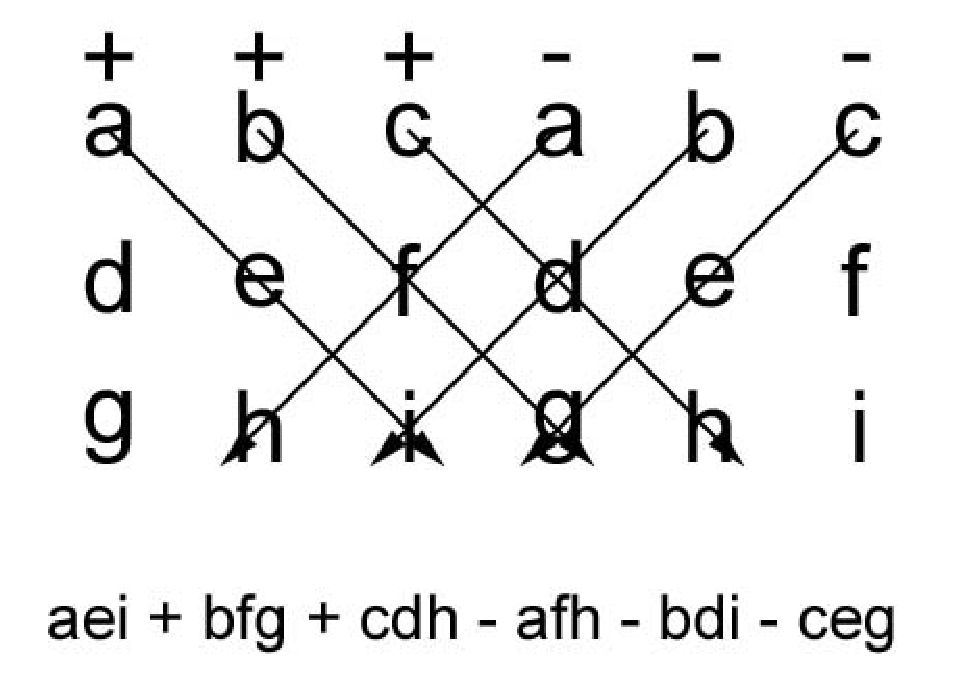
\includegraphics[scale=0.3]{Determinant_3x3-wikipedia.eps}
     \caption{Regra de Sarrus, note que a repetição da $3^a$ coluna não é necessária. Fonte: Wikipedia, citado nas referencias.}
     \label{fig1}
   \end{figure}
%A figura deve ir antes desse texto por causa do label.
Uma forma prática de calcular esse determinante é a \textit{regra de Sarrus}, na qual se copiam as duas primeiras 
colunas da matriz ao final da mesma e se atribuem os sinais de acordo com a figura~\ref{fig1}
   
   \subsection{Determinantes de ordem maior que 3}
   \subsubsection*{Método de Laplace}
   \addcontentsline{toc}{subsubsection}{Método de Laplace}
   \paragraph*{Cofator} O cofator $A_{ij}$ obtido a partir do elemento $a_{ij}$ da matriz A é obtido multiplicando-se o fator $-1^{i+j}$ pelo determinante da matriz A, excluídas a linha i e coluna j. Por exemplo:
\begin{displaymath}
    \text{Seja A=}\begin{bmatrix}
     a & b & c\\d & e & f\\g & h & i
   \end{bmatrix}
\end{displaymath}
   $\text{O cofator }A_{11}=-1^{1+1}\cdot \begin{vmatrix}
     e & f\\h & i
   \end{vmatrix}\quad A_{12}=-1^{1+2}\cdot \begin{vmatrix}
     d & f\\g & i
   \end{vmatrix}$
   
   O método de Laplace consiste em escolher 1 linha (ou coluna) da matriz A e somar os produtos dos elementos da linha (ou coluna) escolhida pelos respectivos cofatores. Usando a matriz $A_{3\times 3}$ definida antes, vamos calcular seu determinante pelo método de Laplace, vou escolher a linha 1 para eliminar:
   \begin{align*}
     det(A)=&a\cdot A_{11}+b\cdot A_{12}+c\cdot A_{13}\\
     &= a\cdot (-1)^2\cdot \begin{vmatrix} e & f\\h & i\end{vmatrix}+b\cdot(-1)^{3}\cdot
      \begin{vmatrix}d & f\\g & i\end{vmatrix}+  c\cdot (-1)^4\cdot \begin{vmatrix}d & e\\g & h\end{vmatrix}
   \end{align*}
   \subsubsection*{Método da triangularização}
	\addcontentsline{toc}{subsubsection}{Método da triangularização}
	
   Este método se baseia na propriedade vista na seção~\ref{prop:det} que diz que o determinante de uma matriz triangular é o produto dos elementos da diagonal principal. Então o trabalho é transformar o determinante da matriz A no determinante de uma matriz triangular usando operações elementares e lembrando que:
   \begin{itemize}
     \item Quando se multiplica uma linha (ou coluna) da matriz A por um real $\lambda $, o determinante da matriz resultante é igual a $\lambda \cdot det(A)$.
     \item Ao permutar 2 linhas ou colunas da matriz A, o determinante da matriz resultante vale $-det(A)$.
     \item Somar à uma linha (ou coluna) de A uma linha (ou coluna) de A multiplicada por um real não altera o valor do determinante de A.
   \end{itemize}
   Um exemplo: Seja A=$\begin{bmatrix}
     1 & 2 &  1 & 2 \\0 &  1 & 2 & 1\\1 &1 &1 &1\\2 & 0& 1 & 3
   \end{bmatrix}$, calcule $det(A)$\\
   Vamos usar o método de Gauss usando os elementos da diagonal principal como pivôs para
 triangularizar este determinante:
   \begin{align*}
    \begin{vmatrix}
      1 & 2 &  1 & 2 \\0 &  1 & 2 & 1\\1 &1 &1 &1\\2 & 0& 1 & 3
    \end{vmatrix}=
    \begin{vmatrix}
      1 & 2 &  1 & 2 \\0 &  1 & 2 & 1\\0 &-1 &0 &-1\\0 & -4& -1 & -1
    \end{vmatrix}=
    \begin{vmatrix}
      1 & 2 &  1 & 2 \\0 &  1 & 2 & 1\\0 &0 &2 &0\\0 & 0& 7 & 3
    \end{vmatrix}=
    \begin{vmatrix}
      1 & 2 &  1 & 2 \\0 &  1 & 2 & 1\\0 &0 &2 &0\\0 & 0& 0 & 3
    \end{vmatrix}=6
   \end{align*}
Neste exemplo sempre somamos o produto de uma linha por um número real à outra linha, e portanto
o valor do determinante não é alterado. Um caso um pouco mais complicado:
Calcular:$ \begin{vmatrix} 0 & 1 & 2 \\ 1 & 4 & 3 \\ 2 & 2 & 2 \end{vmatrix}$\\
Primeiro vou trocar de lugar a $1^a$ com a $2^a$ linhas:
\[\begin{vmatrix} 0 & 1 & 2 \\ 1 & 4 & 3 \\ 2 & 2 & 2 \end{vmatrix} =- \begin{vmatrix}  1 & 4 & 3\\0 & 1 & 2  \\ 2 & 2 & 2 \end{vmatrix}=\]
Agora vou colocar o 2 da $3^a$ linha para fora do determinante:
\[=-2 \begin{vmatrix}  1 & 4 & 3\\0 & 1 & 2  \\ 1 & 1 & 1 \end{vmatrix}= \]
Usando o método de Gauss para triângularizar o determinante, resulta:
\[=-2 \begin{vmatrix}  1 & 4 & 3\\0 & 1 & 2  \\ 0 & 0 & 4 \end{vmatrix}= -2 \cdot 4 = -8\]

   \newpage
   
\section{Referencias Bibliográficas}
\begin{enumerate}
  \item Álgebra Linear e Aplicações; Callioli,A. C., Domingues, H. H., Costa, R. C. F., $6^{\underline{a}}$ edição.
  \item http://pt.wikipedia.org/wiki/Determinante
  \item http://mathworld.wolfram.com/MatrixInverse.html - artigo sobre matrizes inversas, em ingles.
\end{enumerate}

\end{document}
